\documentclass{standalone}
\usepackage[usenames,dvipsnames]{xcolor}
\usepackage{tikz}
\usetikzlibrary{decorations.pathreplacing}

\begin{document}

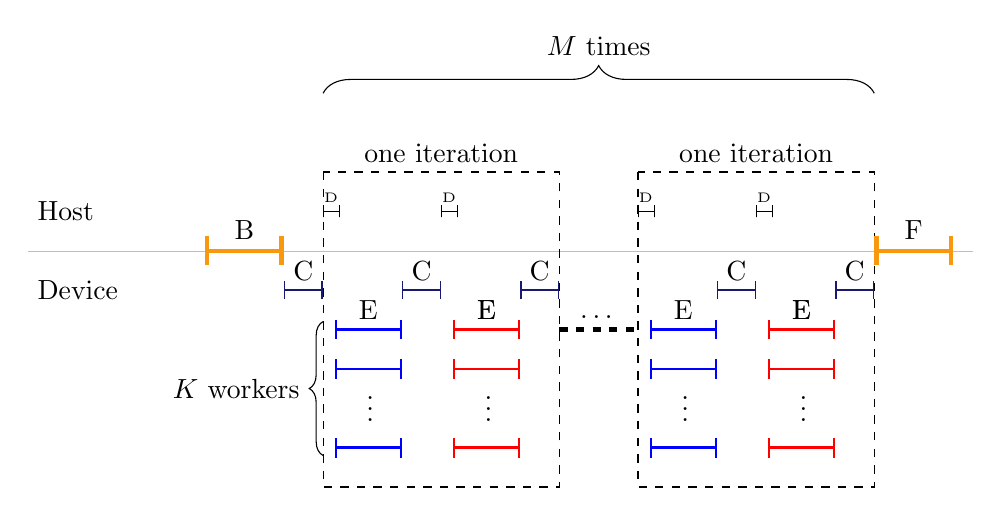
\begin{tikzpicture}[scale=.5]

%% Draw the times sequences

% Host / Device sep
\node at (-2.5, 0) [anchor=west] { Host };
\draw [ultra thin, lightgray] (-2.5, -1) -- (21.5, -1);
\node at (-2.5, -2) [anchor=west] { Device };

% A
%\draw [|-|, thick, ForestGreen] (0, 0) to node [above, black] { A }  (2, 0);

% B
\draw [|-|, ultra thick, YellowOrange] (2, -1) to node [above, black] { B } (4, -1);

% 1st C
\draw [|-|, semithick, MidnightBlue] (4, -2) to node [above, black] { C } (5, -2);

% 1st iter box
\draw [dashed] (5, 1) rectangle (11, -7);
\node at (8, 1) [above] { one iteration };

% 1st sub iter
\draw [|-|, ultra thin] (5, 0) to node [above, font=\tiny] { D } (5.4, 0);
\draw [|-|, thick, blue] (5.3, -3) to node [above, black] { E } (7, -3);
\draw [|-|, thick, blue] (5.3, -4) -- (7, -4);
\node at (6.2, -4.8) {\vdots};
\draw [|-|, thick, blue] (5.3, -6) -- (7, -6);

% K workers
\draw [decorate, decoration={brace, amplitude=5}] (5, -6.2) to node [left=5pt] { $K$ workers } (5, -2.8);

% sync C
\draw [|-|, semithick, MidnightBlue] (7, -2) to node [above, black] { C } (8, -2);

% 2nd sub iter
\draw [|-|, ultra thin] (8, 0) to node [above, font=\tiny] { D } (8.4, 0);
\draw [|-|, thick, red] (8.3, -3) to node [above, black] { E } (10, -3);
\draw [|-|, thick, red] (8.3, -3) to node [above, black] { E } (10, -3);
\draw [|-|, thick, red] (8.3, -4) -- (10, -4);
\node at (9.2, -4.8) {\vdots};
\draw [|-|, thick, red] (8.3, -6) -- (10, -6);

% sync C
\draw [|-|, semithick, MidnightBlue] (10, -2) to node [above, black] { C } (11, -2);

% ... between iter boxes
\draw [ultra thick, dashed] (11, -3) to node [above] { \dots } (13, -3);

% last iter box
\draw [dashed] (13, 1) rectangle (19, -7);
\node at (16, 1) [above] { one iteration };

% 1st sub iter
\draw [|-|, ultra thin] (13, 0) to node [above, font=\tiny] { D } (13.4, 0);
\draw [|-|, thick, blue] (13.3, -3) to node [above, black] { E } (15, -3);
\draw [|-|, thick, blue] (13.3, -4) -- (15, -4);
\node at (14.2, -4.8) {\vdots};
\draw [|-|, thick, blue] (13.3, -6) -- (15, -6);

% sync C
\draw [|-|, semithick, MidnightBlue] (15, -2) to node [above, black] { C } (16, -2);

% 2nd sub iter
\draw [|-|, ultra thin] (16, 0) to node [above, font=\tiny] { D } (16.4, 0);
\draw [|-|, thick, red] (16.3, -3) to node [above, black] { E } (18, -3);
\draw [|-|, thick, red] (16.3, -3) to node [above, black] { E } (18, -3);
\draw [|-|, thick, red] (16.3, -4) -- (18, -4);
\node at (17.2, -4.8) {\vdots};
\draw [|-|, thick, red] (16.3, -6) -- (18, -6);

% sync C
\draw [|-|, semithick, MidnightBlue] (18, -2) to node [above, black] { C } (19, -2);

% brace w/ "M times"
\draw [decorate, decoration={brace, amplitude=10}] (5, 3) to node [above=10pt] { $M$ times } (19, 3);

% F
\draw [|-|, ultra thick, YellowOrange] (19, -1) to node [above, black] { F } (21, -1);

% G
%\draw [|-|, thick, ForestGreen] (21, 0) to node [above, black] { G }  (23, 0);

\end{tikzpicture}


\end{document}
